\documentclass{article}

\usepackage{amssymb}
\usepackage{amsmath}
\usepackage{hyperref}


\usepackage{amsfonts}
\usepackage{booktabs}
\usepackage{siunitx}

\usepackage{graphicx} % Required for inserting images
\usepackage{algpseudocodex}
% \usepackage[preprint]{neurips_2024}
\usepackage[preprint]{neurips_2024}
\begin{document}
\graphicspath{ {Figures/} }

\section{1.1 Exploratory data analysis}

\textbf{REMOVE THESE AUTOMATIC INDICES FROM OVERLEAF CAN BE CONFUSING}
\textbf{WE SHOULD HAVE AN ABSTRACT, add citations as well, website and book from my part.}


\subsection{Basic facts}
We have a dataset that consists of 5471 (n) samples with 4124 (p) columns. The features of our data are all continuous, in a logarithmic scale and they expression levels 
for genes. It is worth mentioning that the dataset is sparse, that is, a lot of cells have many gene expressions that are 0. While it is hard to have an objective measure
of sparsity we can plot average gene expression levels across all our features, see Figure \ref{fig:hist_sparse} below, most genes are non zero for a limited number of cells.



We have 2 distinct classes of cells, the TREG cells and the CD4+T cells. 
These are going to be our labels that we want to classify. We have some class imbalance, the ratio is 6/10 in favour of the CD4+T, 
which is the dominant class. This is going to be important for the models we try to tune as some models have options to adjust for class imbalance.
We will also try the option of tuning the threshold decision for classifying to one cell or another. By default the probabilistic models in Scikit-learn
classify to the positive class if the conditional probability for the given model $\mathbb{P}(\textit{y}|X) > 0.5$\footnote{\href{https://scikit-learn.org/1.5/modules/classification_threshold.html}{see scikit references}}. 
We will tinker with this threshold to try to optimize the F1-Score given our class imbalance.  

\subsection{Visualization and dimensionality redcution}

Both the fact that $n \approx p$ and the fact that the data is sparse point us towards using towards using regularization and feature selection.
The instructions for this problem also make us use PCA with 10 components. To confirm whether the number of components is optimal, we can plot the cumulative sum of the explained variance by each of the components.
As you can see below in Figure \ref{fig:scree}, choosing just the first ten components makes us use a very amount of the total variance.
In Section \ref{sec:1.3} we will try to tune the number of components to get an improved F1-Score.

\begin{figure}[h]
    \centering
    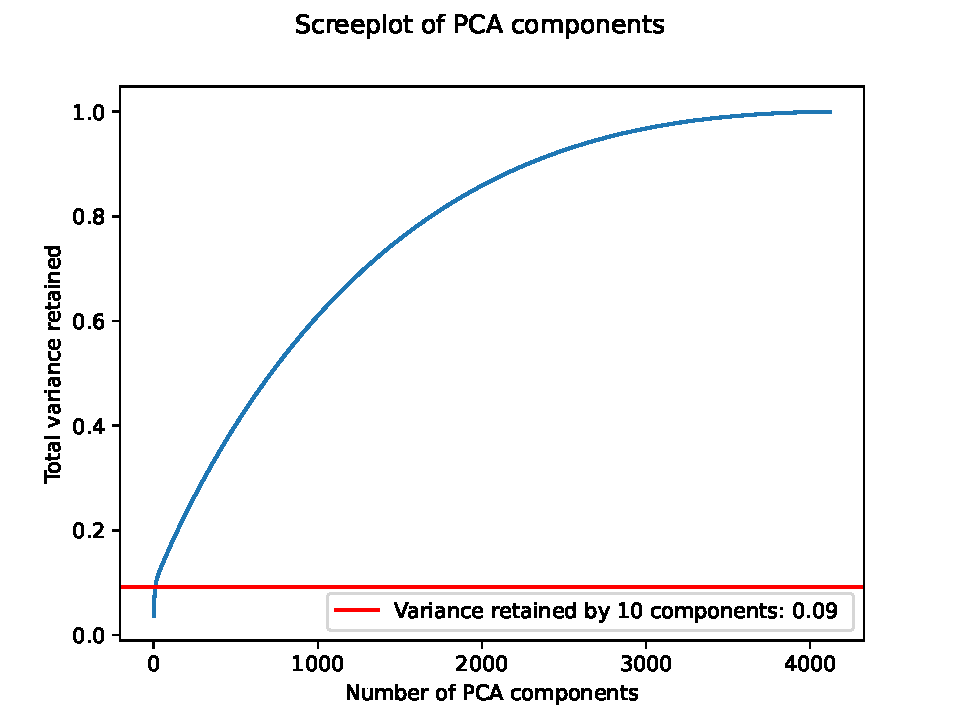
\includegraphics[width=0.8\textwidth]{t11_screeplot.pdf}
    \caption{Scree plot: cumulative sum of PCA components.}\label{fig:scree}
\end{figure}

For completeness, we add Figure \ref{fig:tsne} where we use t-SNE to reduce the dimensionality of the data from 4124 to 2\footnote{ The underlying algorithm is stochastic 
and quite sensitive to how we tune the hyperparameter of perplexity} with the purpose of visualizing the joint distribution (after the t-SNE transformation) of both cells. 
Figure \ref{fig:tsne} shows some separability of the two classes. It also shows some cells of a given clas (TREG) in regions where the density is much higher for the other type of cell (CD4T), maybe we can use this as intuition as to why
in later sections we find it difficult to improve the F1-Score beyond 0.95.


\begin{figure}[h]
    \centering
    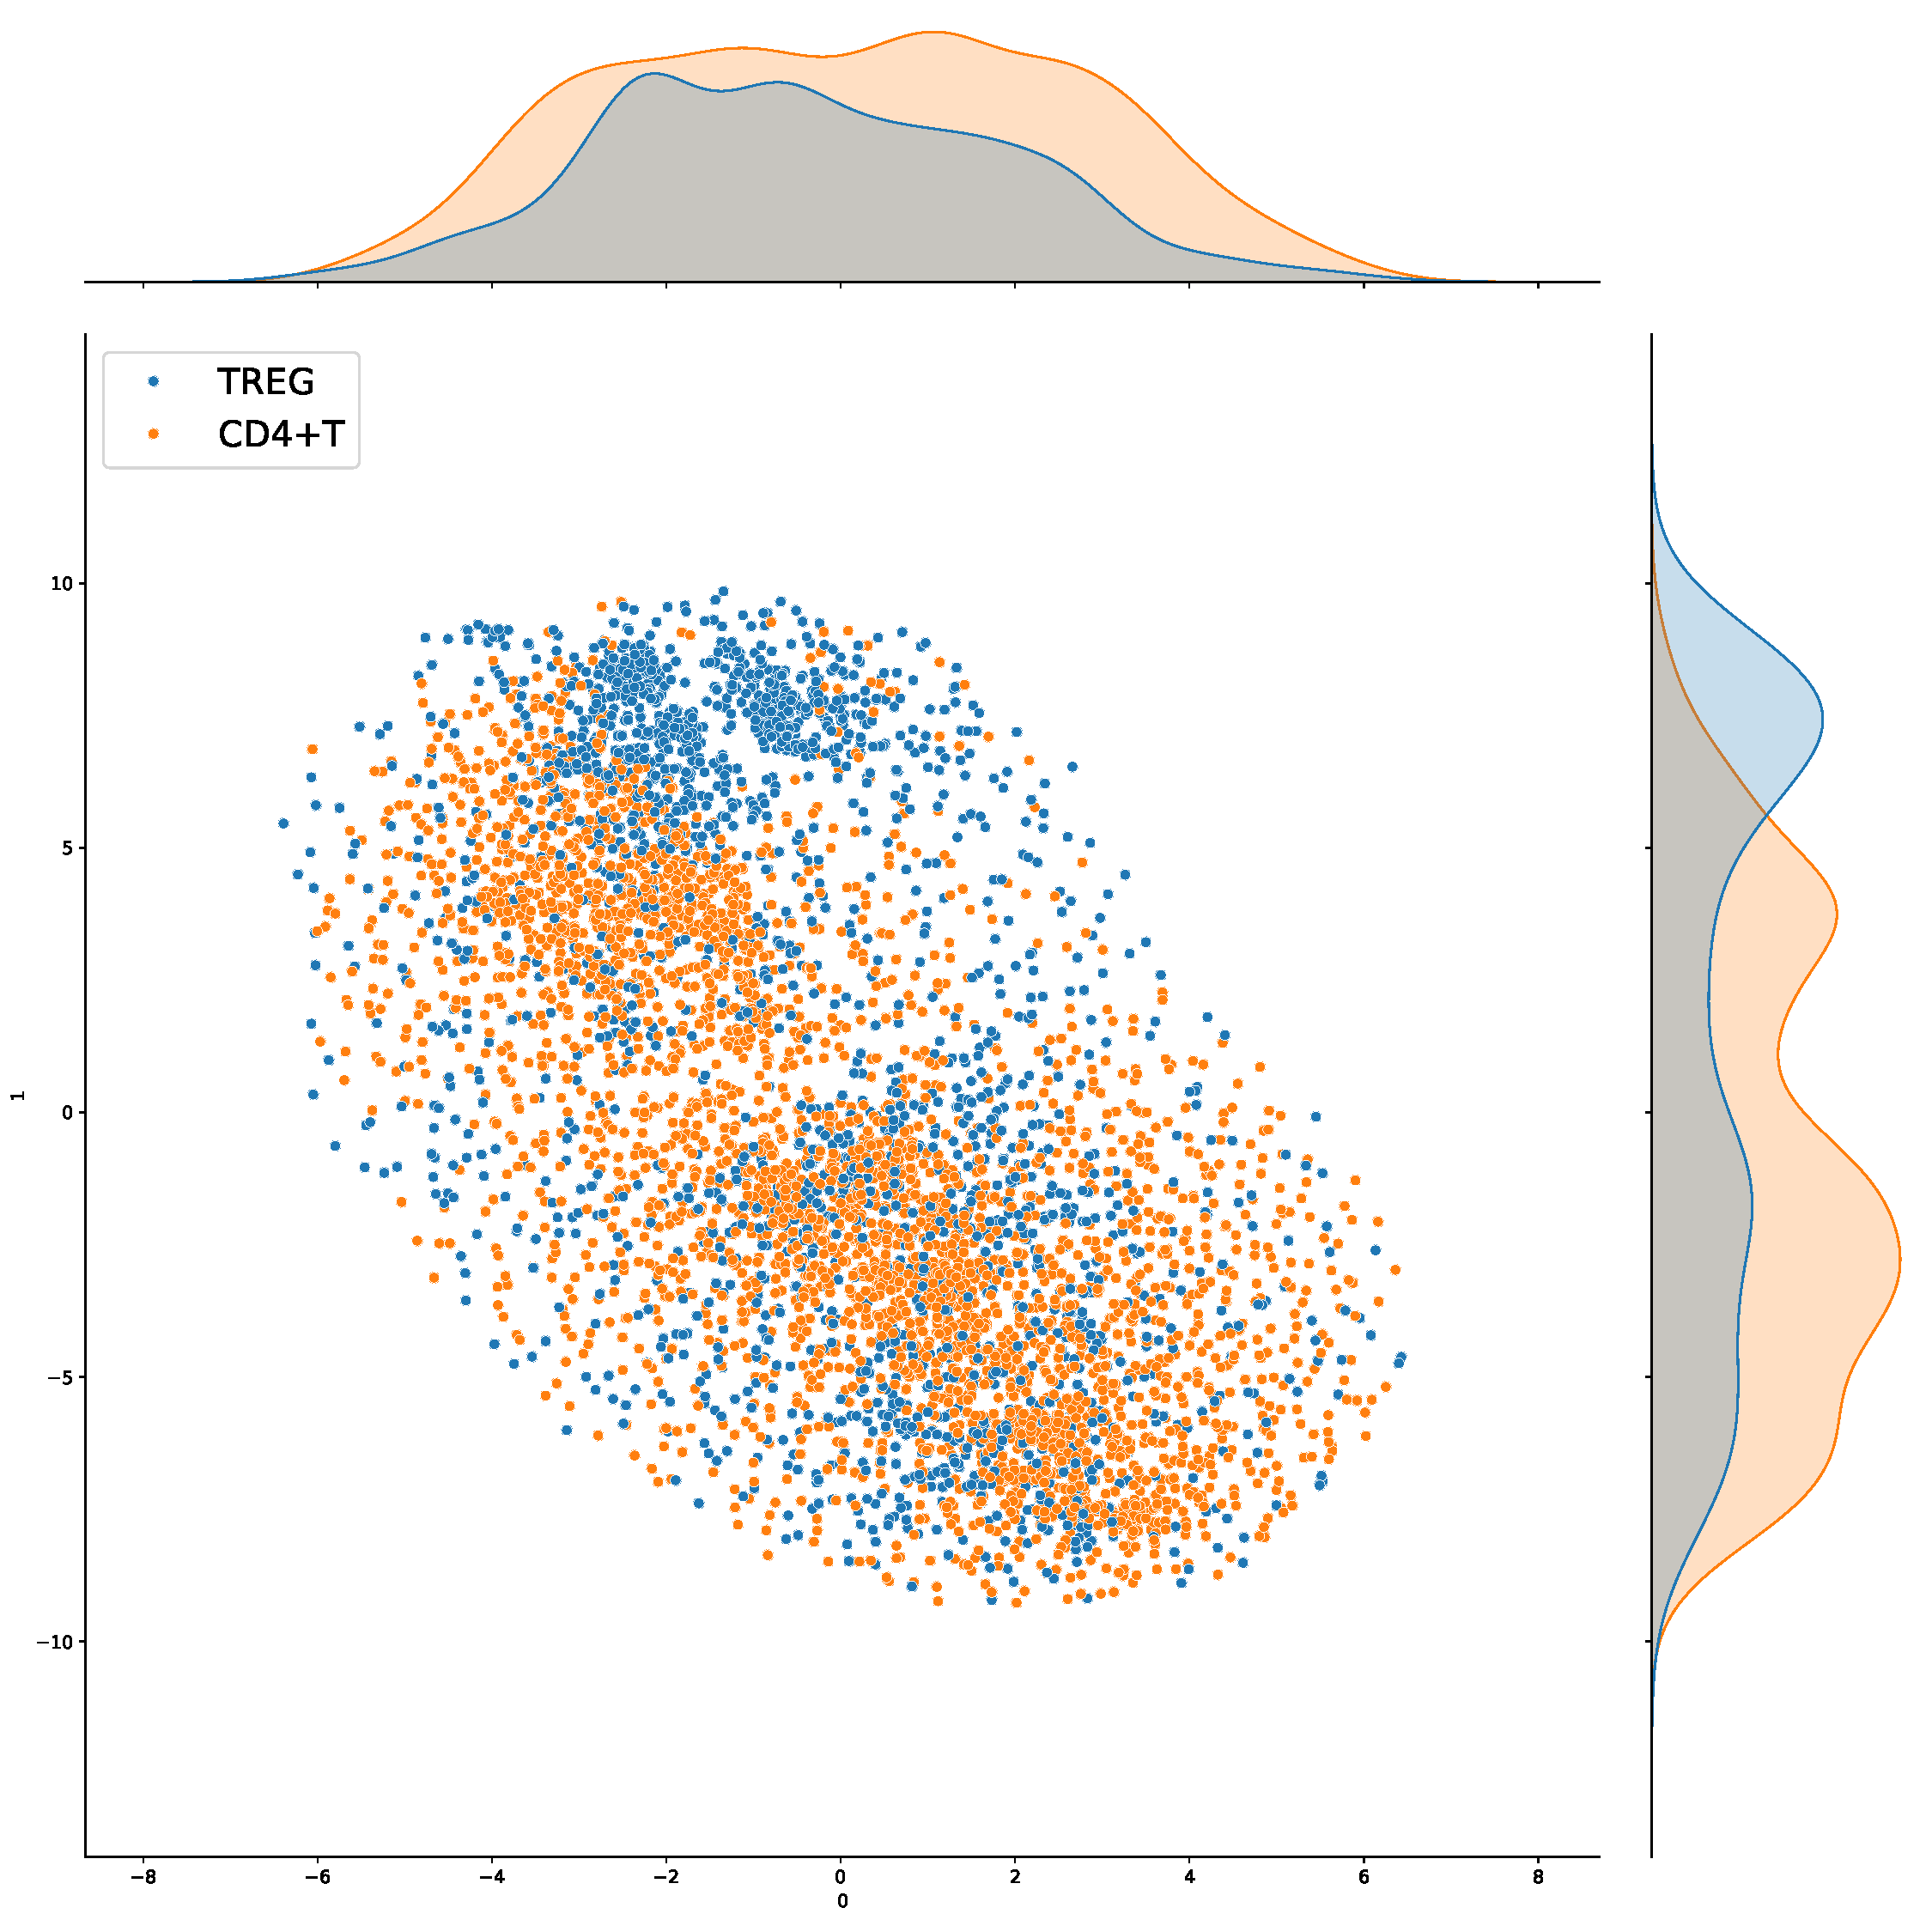
\includegraphics[width=0.8\textwidth]{t11_joint_tsne.pdf}
    \caption{Joint distribution of transformed data by t-SNE}\label{fig:tsne}
\end{figure}
% Make sure we explain why it doesn't work. -> T-sne or something like that.
% Correct way to use t-sne if we have space is to plot different perplexities. TRY DO IT AND JUST MENTION IT IN A NOTE.
% \section{Training baseline models and hypertuning}

\section{1.2 Training, tuning and evaluating baseline models.}
This section is split into two parts, the first part describes our code from Python at a high-level. It focuses on some of scikit-learn procedures to streamline the analysis 
and guarantee good test performance. Then we move to explain which parameters we tune to improve the performance of the baseline models.

\subsection{Using the scikit-learn toolkit.}
Because we are going do to some hyperparameter tuning we first need to split the data into a test and train subset -this is needed because we tuned some hyperparameters, if not an estimate of test error obtained through cross validation should be valid -\footnote{The \href{https://scikit-learn.org/1.5/modules/cross_validation.html}{scikit documentation} contain a very understandable graph of the workflow.}

To do the hyperparameter tuning we implemented grid search\footnote{The scikit documentation on \href{https://scikit-learn.org/1.5/modules/grid_search.html}{grid search.}
} which is a brute force approach that consists of trying all hyperparameter combinations specified by the researcher. 
We use the training set for a given set of parameters, we use cross validation -a part of our training data is left out as a validations set, the model is trained on the rest of the training data and we get a validation error estimate, this process is repeated 5 times - and obtain an estimate of the metric we are trying to optimize over.
We iterate over all parameter combinations and pick the one that maximizes the metric we choose (in part 1 it was F1 score).

Some models need the data to be standarized, and we are also asked to use PCA, we therefore make use of pipelines \footnote{The scikit library has great documentation:
\href{https://scikit-learn.org/stable/modules/generated/sklearn.pipeline.Pipeline.html}{Pipeline} includes some case uses.}, which are a sequence of data preprocessing steps with a final estimator. Using this 
streamlines our analysis and avoids some \href{https://scikit-learn.org/stable/common_pitfalls.html}{common pitfalls.}
Example: Our cross validation estimator has selected a random subset of the training data, then the pipeline will: Standarize the data $\rightarrow$ Apply PCA $\rightarrow$ Fit the classifier on the preprocessed data.

Finally, throughout our analysis we tried to set a random seed so that our results are reproducible. We forgot about randomness in the PCA algorithm used by scikit-learn, while the exact numbers may change, the overall picture and decision making is not affected.

\subsection{Hyperparameter tuning the baseline models.}
We focus on tuning the models without PCA, as that is where most of the gains can be made. Due to the relatively high dimensionality of the
data some models are underperfoming if we use all the features avalable. In contrast even the out-of-the-box models without hyperparameter tuning 
perform really well when training on the first 10 components of the PCA. Therefore we compare the tuned models without PCA to the untuned models with PCA. 
Next we show what we tuned and the results we obtained.

\subsubsection{What did we tune?}

For the first 3 models -\textit{LDA, Logistic regression and QDA}- the tuning is mostly focused on imposing strong penalization mechanisms, such as lasso, ridge or elastic net.

For \textit{k-NN}, there are a lot of interesting parameters. We search across different numbers of neighbors. We also tune across rules to determine who the nearest
neighbors are. To achieve this we use the Minkowski(p) distance, this is a distance that nests the classical euclidean (Minkowski($p_1$)) and manhattan distances (Minkowski($p_2$)), so we search across p to try different distances.
Finally we also try to compute the decision rule in different weights, the default where all neighbors have the same weight in the vote and one where the votes from the closest neighbors within the neighborhood carry more weight.

For \textit{Support Vector Machine}, we tune across different kernels and regularization strenghts. The default uses the radial/gaussin kernel, we also try to use linear kernels as well as some others we haven't seen in class.

For \textit{Random Forests} our grid search is not extensive, we tune the criterion made to determine the quality of a split (gini and entropy), the number of trees in the forest and the number of features a tree in the forest will choose from.
It is worth mentioning that we considered pruning, as we saw the method in class, however we decide against it as it would be computationally expensive.

For \textit{Gradient Boosted Decision Trees (GBDT)} we consider different loss functions, number of iterations, learning rates, as well as the depth and features used by the trees. 
We also set an early stopping rule as this grid search is computationally expensive.
For other models the tuning parameters are mostly self explanatory, in this case it is more complex.
For intuition let us remember that this is similar to AdaBoost, learning determines how new iterations influence the final vote and the tree complexity should be tuned to avoid overfitting.
If we run too many iterations with a deep tree we might overfit, while if we run too few iterations on shallow trees, our performance may be suboptimal.
Finding the optimal between iterations, learning and tree complexity is complex.

Finally, across our tuning, we  use tuning paramters related to class weights were available. As while the classes are not as imbalanced as in Task 2, there is some imbalance in favour of the CD4+T.
    


\subsubsection{Analysis of results}

We compare our fully tuned models without PCA to out of the box models with PCA. As you can see from Table 1 below
out-of-box with PCA have similar or better performance to the ones we fully tune without PCA.
The models most affected by PCA are LDA, QDA and \textit{k-NN}. Using PCA improves the perfomance of QDA and K-NN dramatically. 
For Logistic regression and LDA, the performance is not improved too much as the optimal models from the tuning already contain severe forms of regularization,
which is very similar in spirit to what PCA is doing. SVM is consistently great. Random forest gets a small improvement from the PCA and GBDT lowers the performance slightly,
although both these models are consistent in making very good predictions.

\begin{table}[h]
    \centering
    \begin{tabular}{lSSSSl}
        \toprule
        {Model} & {Accuracy} & {Balanced Acc.} & {AUC} & {F1 Score} & {Confusion Matrix} \\
        \midrule
        LDA & \textbf{0.965} & \textbf{0.956} & 0.993 & \textbf{0.951} & \([687, 6], [32, 370]\) \\
        LOGIT & 0.958 & 0.954 & 0.993 & 0.942 & \([672, 21], [25, 377]\) \\
        QDA & 0.367 & 0.500 & 0.500 & 0.537 & \([0, 693], [0, 402]\) \\
        KNN & 0.788 & 0.777 & 0.874 & 0.718 & \([567, 126], [106, 296]\) \\
        SVM & 0.956 & 0.953 & 0.993 & 0.940 & \([669, 24], [24, 378]\) \\
        RF & 0.943 & 0.924 & 0.993 & 0.917 & \([690, 3], [59, 343]\) \\
        GBDT & 0.963 & 0.955 & \textbf{0.994} & 0.949 & \([684, 9], [31, 371]\) \\ \midrule
        \textit{With PCA} \\\midrule
        LDA & 0.950 & 0.936 & 0.994 & 0.928 & \([685, 8], [47, 355]\) \\
        LOGIT & 0.966 & 0.965 & 0.994 & 0.954 & \([672, 21], [16, 386]\) \\
        QDA & 0.960 & 0.958 & 0.993 & 0.946 & \([669, 24], [20, 382]\) \\
        KNN & 0.928 & 0.911 & 0.956 & 0.896 & \([675, 18], [61, 341]\) \\
        SVM & \textbf{0.967} & \textbf{0.966} & \textbf{0.994} & \textbf{0.956} & \([672, 21], [15, 387]\) \\
        RF & 0.957 & 0.947 & 0.989 & 0.940 & \([683, 10], [37, 365]\) \\
        GBDT & 0.947 & 0.938 & 0.990 & 0.926 & \([673, 20], [38, 364]\) \\
        \bottomrule
    \end{tabular}
    \caption{Fully tuned models with PCA vs out-of-box with PCA.}
    \label{tab:metrics}
\end{table}



\section{Our 3 models} \label{sec:1.3}
We tried 3\footnote{We tried more than 3 but settled on these 3 because they showcase very different methods.} simple approaches of some things
we saw in class and from our learning in the baseline models. We implemented the AdaBoost from class and tuned it, tinkered with the decision thresholds and we 
tried different numbers of PCA components with an out-of-box SVM. None of our approaches let us \textbf{consistenly} improve to F1 scores of 0.96 or 0.97
\footnote{Due to this we omit showing these results, they can be found in the notebook for completeness.}. 

\begin{itemize}
    \item AdaBoost, just because we have seen it in class and it could be interesting.
    \item Threshold optimization: https://towardsdatascience.com/tune-in-decision-threshold-optimization-with-scikit-learns-tunedthresholdclassifiercv-7de558a2cf58
    \item SVM with pca optimization.
\end{itemize}

\begin{figure}[h]
    \centering
    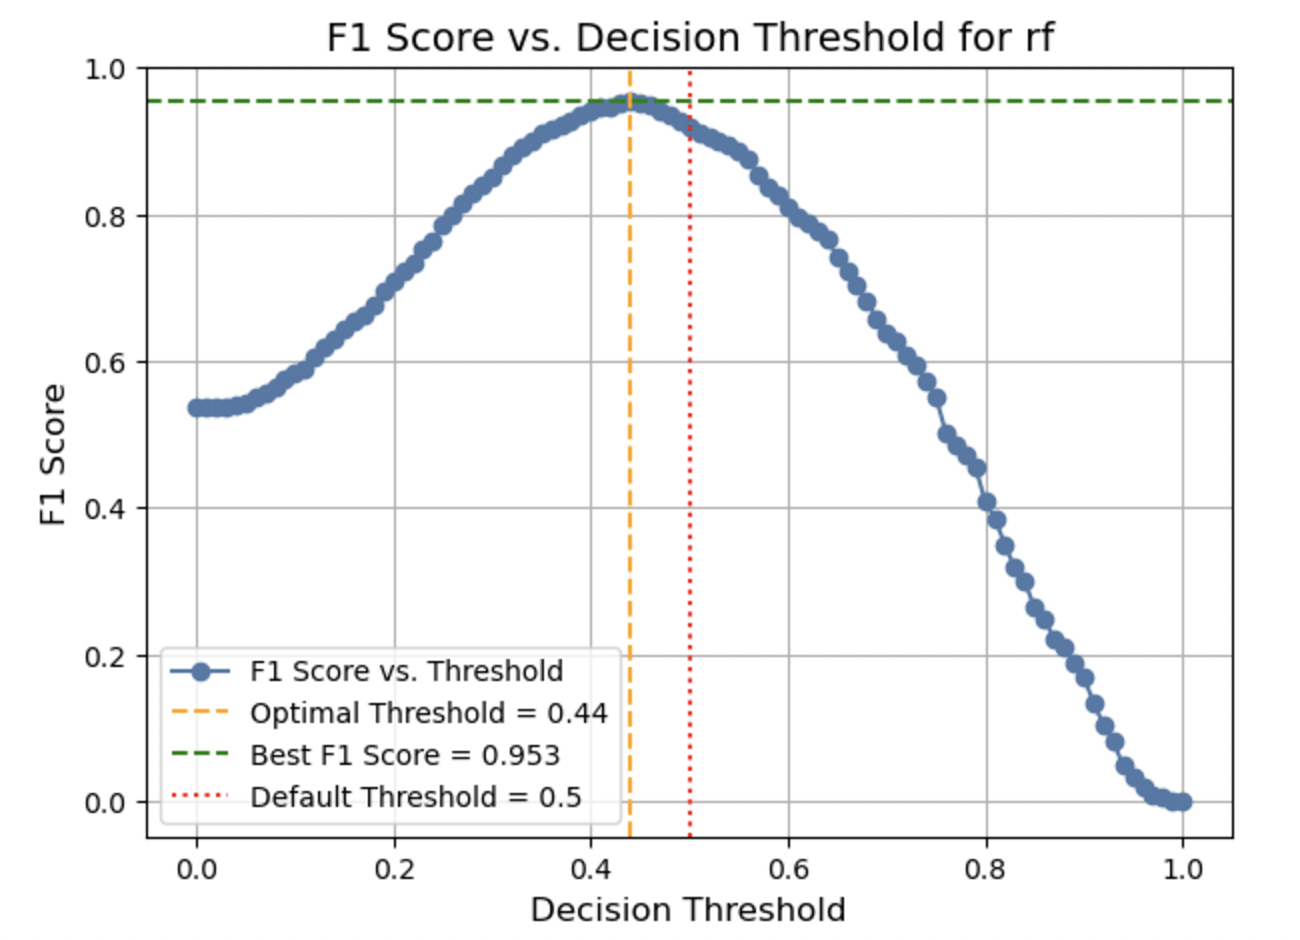
\includegraphics[width=0.8\textwidth]{RF_THRESHOLD_DEF.png}
    \caption{Thresholding example with a random forest model.}\label{fig:thresh_rf}
\end{figure}
\subsection{Our final predictor:}

\end{document}